\chapter{Literature Review and Related Work}
\label{chap:relatedworks}

In this chapter, describe other solutions/research that address the
same topic as your project. If you are working on a software project, create a
list of alternative solutions and analyze them in the competitor analysis section.
If you are working on a research project, describe your related work research in
the literature review section.

\section{Competitor Analysis}
\label{section:competitor-analysis}

% //#TODO: place table here
\begin{figure}[h]
    \centering
    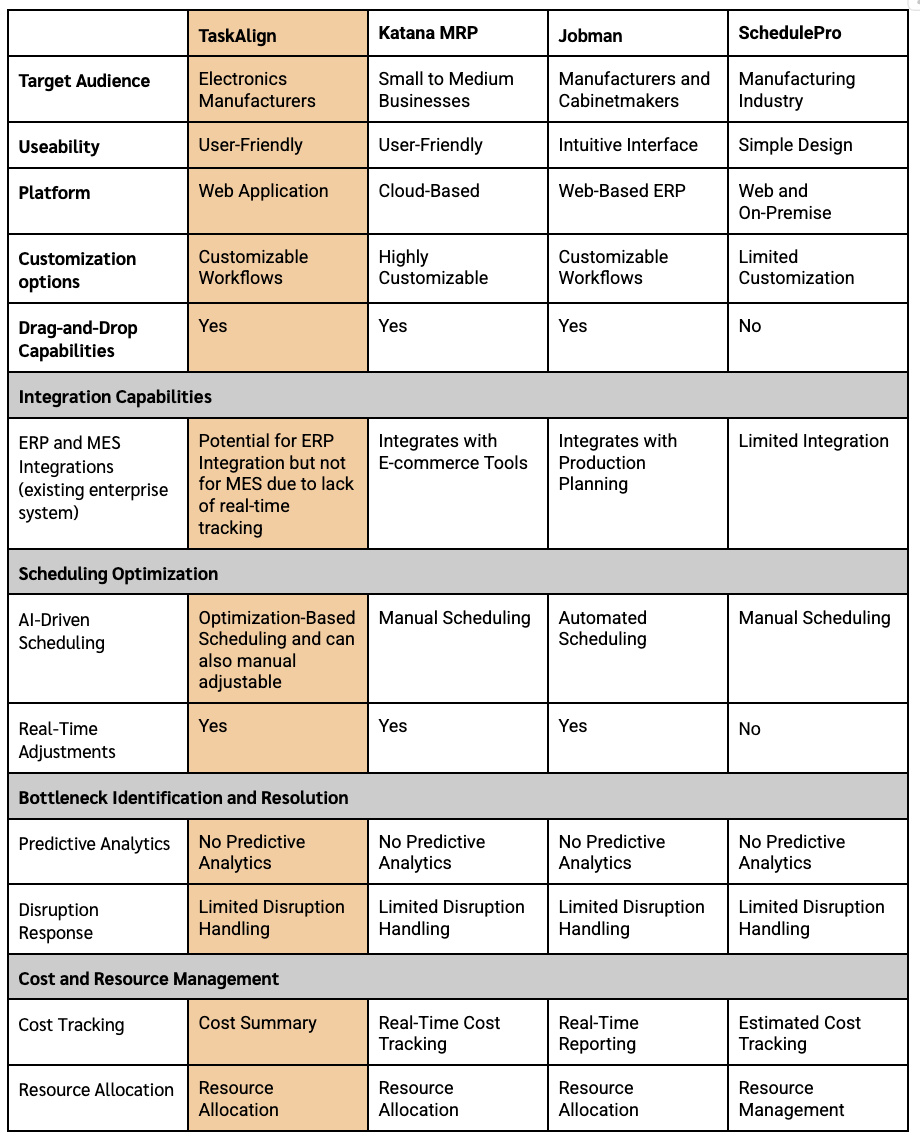
\includegraphics[width=0.5\textwidth]{examples/competitor.png}
    \caption{Competitor Analysis Table} 
\end{figure}

TaskAlign is a task scheduling system designed specifically for electronics manufacturers. Unlike our competitors, TaskAlign utilizes a scheduling system approach to optimize machine usage and workforce allocation. This feature allows TaskAlign to prevent potential bottlenecks and optimize the schedules plan, ensuring efficient production. TaskAlign also stands apart due to its reduced production time. TaskAlign provides potential for integrations with existing ERP systems by providing optimized task schedules that align with production planning and resource management, unlike SchedulePro which offers limited integration. TaskAlign's highly customizable workflows allow for flexible adjustments tailored to electronics manufacturing processes, offering greater flexibility than Katana MRP and Jobman.


\section{Literature Review}
\label{section:literature-review}


\subsection{Current Approaches to Production Scheduling}

Production scheduling is a critical component of manufacturing operations that directly impacts efficiency, resource utilization, and overall productivity. Traditional production scheduling often relies heavily on human experience and manual planning, which can lead to suboptimal resource allocation and inefficiencies in complex manufacturing environments \cite{alander2024}. As manufacturing systems become increasingly complex with multiple interconnected processes, traditional scheduling methods struggle to maintain efficiency.

Chen et al. \cite{chen2023} define task scheduling as a real-time process where multiple task attributes must be considered simultaneously while different tasks are processed in parallel. This complexity is particularly evident in microservice-oriented industrial software, where multiple business processes must be executed concurrently. Their research highlights that effective scheduling must account for various characteristics, including strict real-time requirements, the coexistence of independent tasks and workflows, importance-based task attributes, and multi-task processing capabilities.

\subsection{Optimization-Based Scheduling Methods}

Optimization algorithms play a significant role in modern production scheduling approaches. Alander and Hjalmarsson \cite{alander2024} demonstrated that Genetic Algorithms (GAs) can effectively optimize production sequences, achieving up to 42\% reduction in total processing time compared to alphabetically ordered sequences. Their work emphasizes that even simple randomization of production sequences can improve efficiency by 12--17\%, highlighting the inefficiency of simplistic scheduling approaches.

Various algorithms have been developed for production scheduling optimization, including:

\begin{itemize}
    \item \textbf{First Come First Serve Algorithm (FCFS)}: Tasks are processed in order of arrival, which is simple but often inefficient.
    \item \textbf{Earliest Deadline First Algorithm (EDF)}: Prioritizes tasks with the earliest deadlines.
    \item \textbf{Least Laxity First Algorithm (LLF)}: Schedules tasks based on their laxity (deadline minus processing time).
    \item \textbf{Fixed Priority Scheduling Algorithm (FPS)}: Assigns static priorities to tasks \cite{chen2023}.
\end{itemize}

However, these traditional algorithms often fail to consider the complex constraints and multiple objectives present in modern manufacturing environments. Chen et al. \cite{chen2023} proposed a Dynamic Importance-aware Online Scheduling Algorithm (DIOS) that ranks and schedules tasks based on a comprehensive importance function considering inherent task importance, deadline constraints, and critical path factors. Their experimental results demonstrated that DIOS significantly outperformed traditional algorithms in both power system and factory production management scenarios.

\subsection{Smart Manufacturing Scheduling}

The concept of Smart Manufacturing Scheduling (SMS) represents an evolution in production scheduling, leveraging digital technologies to achieve higher levels of automation and autonomy. According to Boza et al. \cite{serranoruiz2023}, SMS integrates Digital Twin (DT) technology with Zero-Defect Manufacturing (ZDM) principles to facilitate self-managing scheduling systems that reduce or eliminate human intervention.

Digital Twin technology enables real-time simulation and optimization of manufacturing processes, allowing for dynamic adjustments in response to disruptions. This capability is particularly valuable for addressing the challenges of complex production environments with varying constraints and requirements \cite{serranoruiz2023}.

\subsection{Constraints and Resource Considerations}

Effective production scheduling must account for various constraints and resource limitations. Alander and Hjalmarsson \cite{alander2024} explored the impact of space constraints and fixtures on production efficiency, finding that optimization becomes increasingly important as resource constraints tighten. Their experiments with varying numbers of concurrent products demonstrated that scheduling efficiency is significantly affected by resource constraints, with optimization benefits becoming more pronounced under tighter constraints.

Chen et al. \cite{chen2023} introduced resource reservation and preemptive scheduling mechanisms to enhance scheduling efficiency. Their resource reservation mechanism ensures that resources needed for high-importance tasks are not allocated to lower-priority tasks, while preemptive scheduling allows urgent tasks to interrupt ongoing less critical tasks. These mechanisms were shown to improve the real-time responsiveness of scheduling systems, particularly in scenarios with time-critical tasks.

\subsection{Adaptive and Real-Time Scheduling}

Modern manufacturing environments require scheduling systems that can adapt to changing conditions and constraints. Chen et al. \cite{chen2023} incorporated an online adaptive tuning method in their DIOS algorithm to continuously adjust scheduling parameters based on real-time conditions, ensuring robust performance under dynamic manufacturing scenarios.